%!TEX program = <xelatex>
\documentclass[xetex]{beamer}
% \documentclass[draft, xetex]{beamer}

		% Iclude packages and commands used text-wide.	
%%%%%%%%%%%%%%%%%%%%%%%%%%%%%%%%%%%%%%%%%%%%%%%%%%%%%%%%%%%%%%%%%%%%%%%%%%%%%%%%%%%%%%%%%%%%%%%%%%%%%%%%%%%

\usepackage{mystyle}

		% Presentation settings.
%%%%%%%%%%%%%%%%%%%%%%%%%%%%%%%%%%%%%%%%%%%%%%%%%%%%%%%%%%%%%%%%%%%%%%%%%%%%%%%%%%%%%%%%%%%%%%%%%%%%%%%%%%%


		% Title
	\title[ETD]{Mass Spectrometry Analysis of Proteins Using Electron Transfer Dissociation}
	\subtitle{Statistical Model}

	%\beamerdefaultoverlayspecification{<+->}
	\date{17 October 2013} 
	\author[Matteo]{Mateusz Łącki}
	\institute[UW]{Uniwersytet Warszawski}
	\titlegraphic{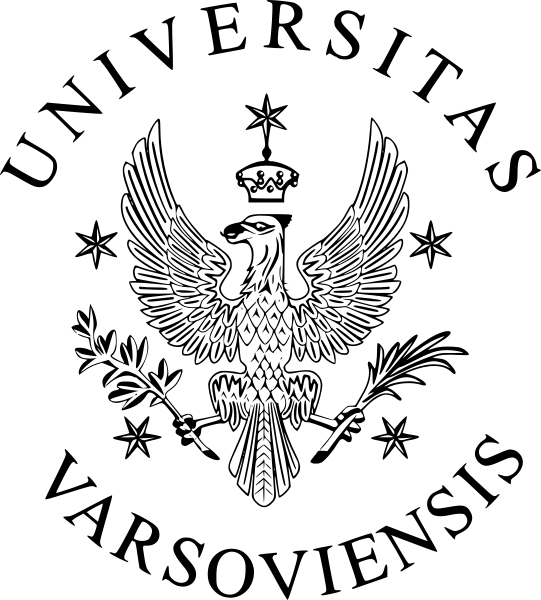
\includegraphics[scale=.10 , keepaspectratio]{./picts/eagle3.png}}
	
		% The document
%%%%%%%%%%%%%%%%%%%%%%%%%%%%%%%%%%%%%%%%%%%%%%%%%%%%%%%%%%%%%%%%%%%%%%%%%%%%%%%%%%%%%%%%%%%%%%%%%%%%%%%%%%%	

\begin{document}

	\fontspec[Numbers={OldStyle}]{Linux Libertine O}

	%%%%%%%%%%%%%%%%%%%%%%%%%%%%%%%%%%%%%%%%%%%%%%%%%%%%%%%%%%%%%%

	\begin{frame}
		\titlepage
	\end{frame}

\section[Motivation]{What is our motivation?}		
	%%%%%%%%%%%%%%%%%%%%%%%%%%%%%%%%%%%%%%%%%%%%%%%%%%%%%%%%%%%%%%%%%%
	\framedGraphic{Data from a Mass Spectrometer for a given substance.}{./picts/inputData.png}
	%%%%%%%%%%%%%%%%%%%%%%%%%%%%%%%%%%%%%%%%%%%%%%%%%%%%%%%%%%%%%%%%%%
	\begin{frame}\frametitle{Project massTodon: Debriefing}
		\begin{itemize}
			\item Mass Spectrometer 
			\begin{itemize}
				\item Evaluation of chemical composition of molecules
				\item Measurements
				\begin{itemize}
					\item[$\star$] $\Big\{ \frac{\text{Mass}_j}{\text{Charge}_j}, \text{Intensity}_j \Big\}_j^{J}$ 
				\end{itemize}
			\end{itemize}
			\item We use MS/MS instrument
			\begin{itemize}
				\item Coupling two mass specs
				\item Filtering specific mass to charge 
				\item Use of the ETD instrument 
			\end{itemize}
			\item Why all that?
			\begin{itemize}
				\item Study structure of peptides by inducing cleavages
			\end{itemize}
		\end{itemize}
	\end{frame}

	\framedGraphic{Inducing Cleavages}{./picts/puzzles.pdf}
	%%%%%%%%%%%%%%%%%%%%%%%%%%%%%%%%%%%%%%%%%%%%%%%%%%%%%%%%%%%%%%%%%%
	\begin{frame}\frametitle{Today's Agenda}
		\tableofcontents
	\end{frame}

%%%%%%%%%%%%%%%%%%%%%%%%%%%%%%%%%%%%%%%%%%%%%%%%%%%%%%%%%%%%%%%%%%		
\section[Model]{Statistical Modelling}
%%%%%%%%%%%%%%%%%%%%%%%%%%%%%%%%%%%%%%%%%%%%%%%%%%%%%%%%%%%%%%%%%%
	\begin{frame}\frametitle{Multinomial Model}
		    
		\begin{itemize}
			\item What is being explained?
			\begin{itemize}
				\item Distributions of masses 
				\item Deviations from monoisotopic peaks
			\end{itemize}
		\end{itemize}

		\begin{center}
			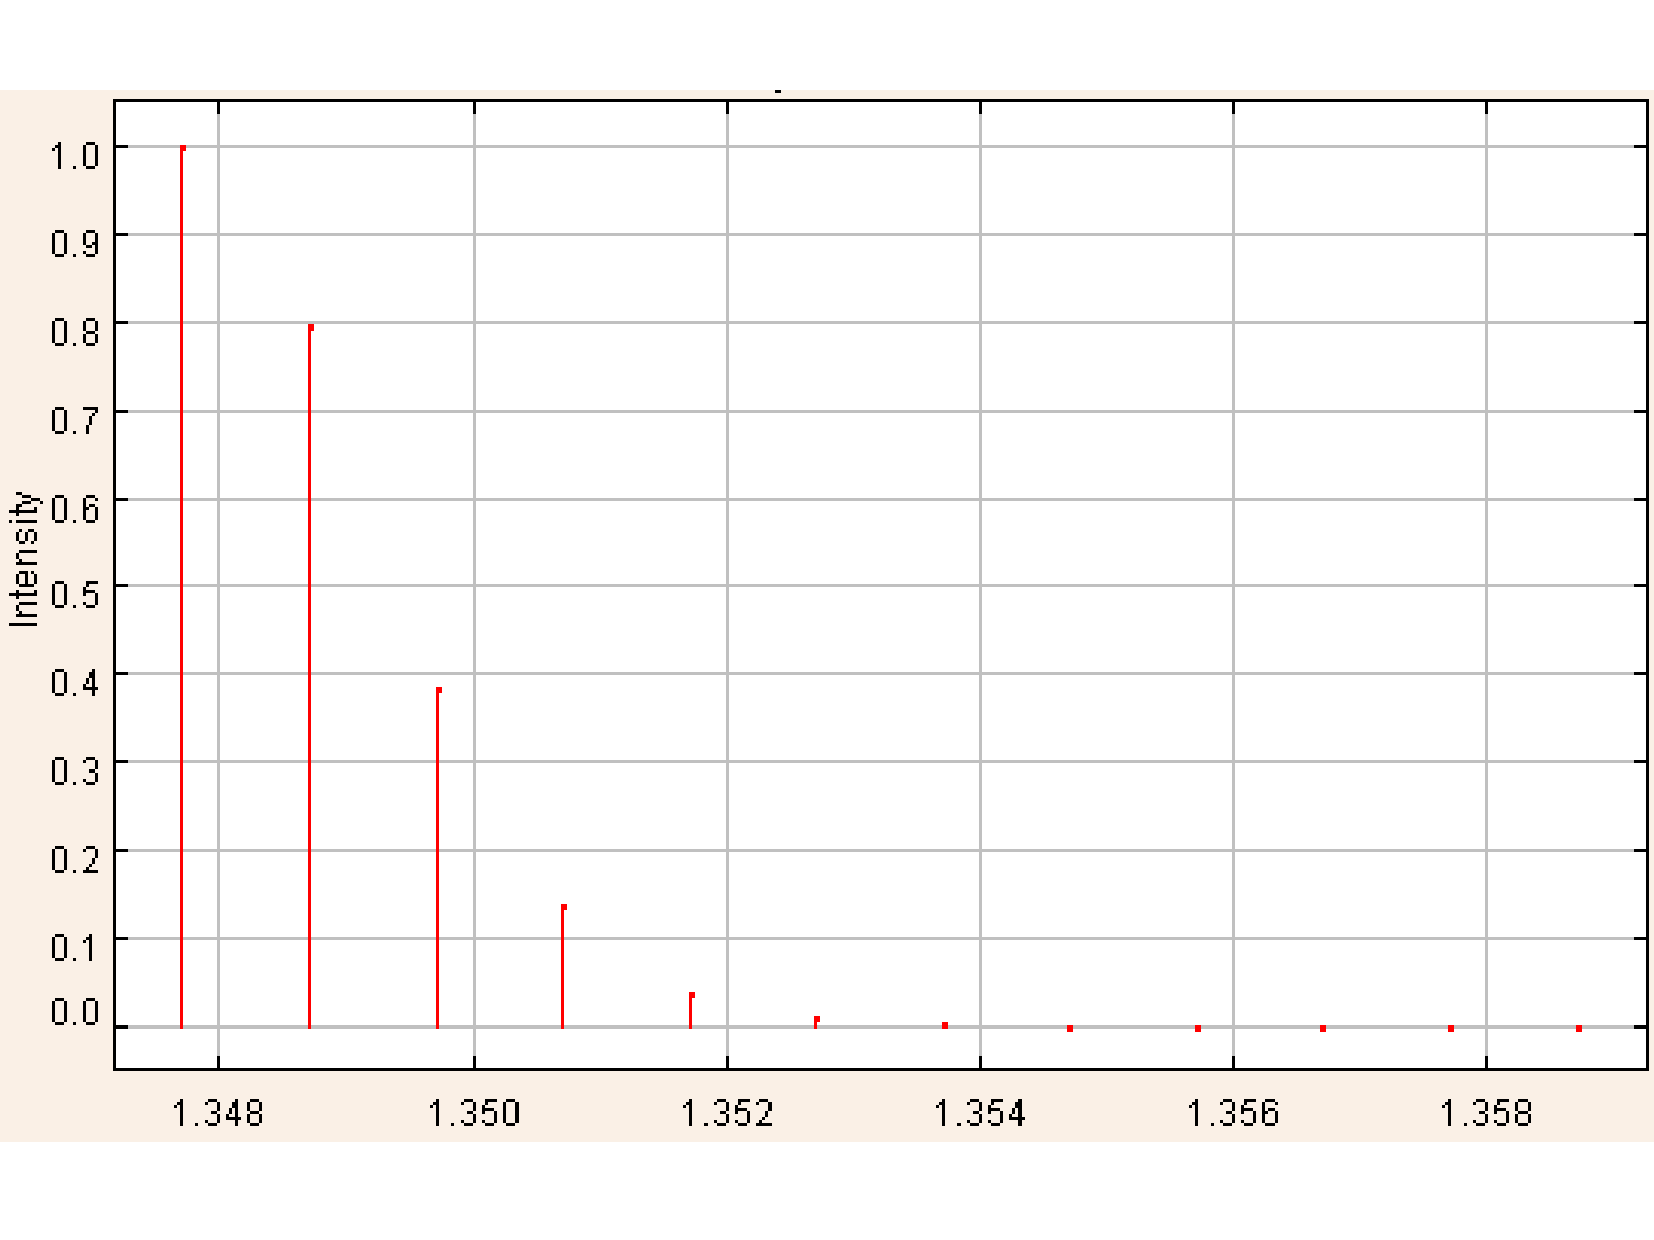
\includegraphics[height=.5\textheight, keepaspectratio]{./picts/realMassDistribution.pdf}
		\end{center}
	\end{frame}	

	%%%%%%%%%%%%%%%%%%%%%%%%%%%%%%%%%%%%%%%%%%%%%%%%%%%%%%%%%%%%%%%%%%
	\begin{frame}\frametitle{Multinomial Model}

		\begin{itemize}
			\item Modelling isotope distributions
			\begin{itemize}
				\item $\prob( \cem{^{16}O} ) = 99.757$
				\item $\prob( \cem{^{17}O} ) = 0.038$
				\item $\prob( \cem{^{18}O} ) = 0.205$
			\end{itemize}
			\item Molecule = \molecule
			\item Assumptions
			\begin{itemize}
				\item Isotope variant of a single atom from \molecule  (e.g. \ce{C}) independent of isotope variants of other atoms
				\begin{itemize}
					\item[i.e.]  for a molecule with 2 atoms
				\end{itemize}				  
				$$\prob( \cem{^{13}C ^{17}O} ) = 
					\prob( \cem{^{13}C} ) \times \prob( \cem{ ^{17}O} ) $$
				\item We cannot discern among isomers
				$$ \cem{^{13}C ^{17}O ^{17}O} \simeq \cem{^{17}O ^{13}C ^{17}O} \simeq \cem{ ^{17}O ^{17}O ^{13}C }$$	
			\end{itemize}
		\end{itemize}

	\end{frame}

	%%%%%%%%%%%%%%%%%%%%%%%%%%%%%%%%%%%%%%%%%%%%%%%%%%%%%%%%%%%%%%%%%%
	\begin{frame}\frametitle{Multinomial Model}
			
		\begin{itemize}
			\item Chemical compound = list of sets of atoms 
			
		\end{itemize}
		\begin{center}
			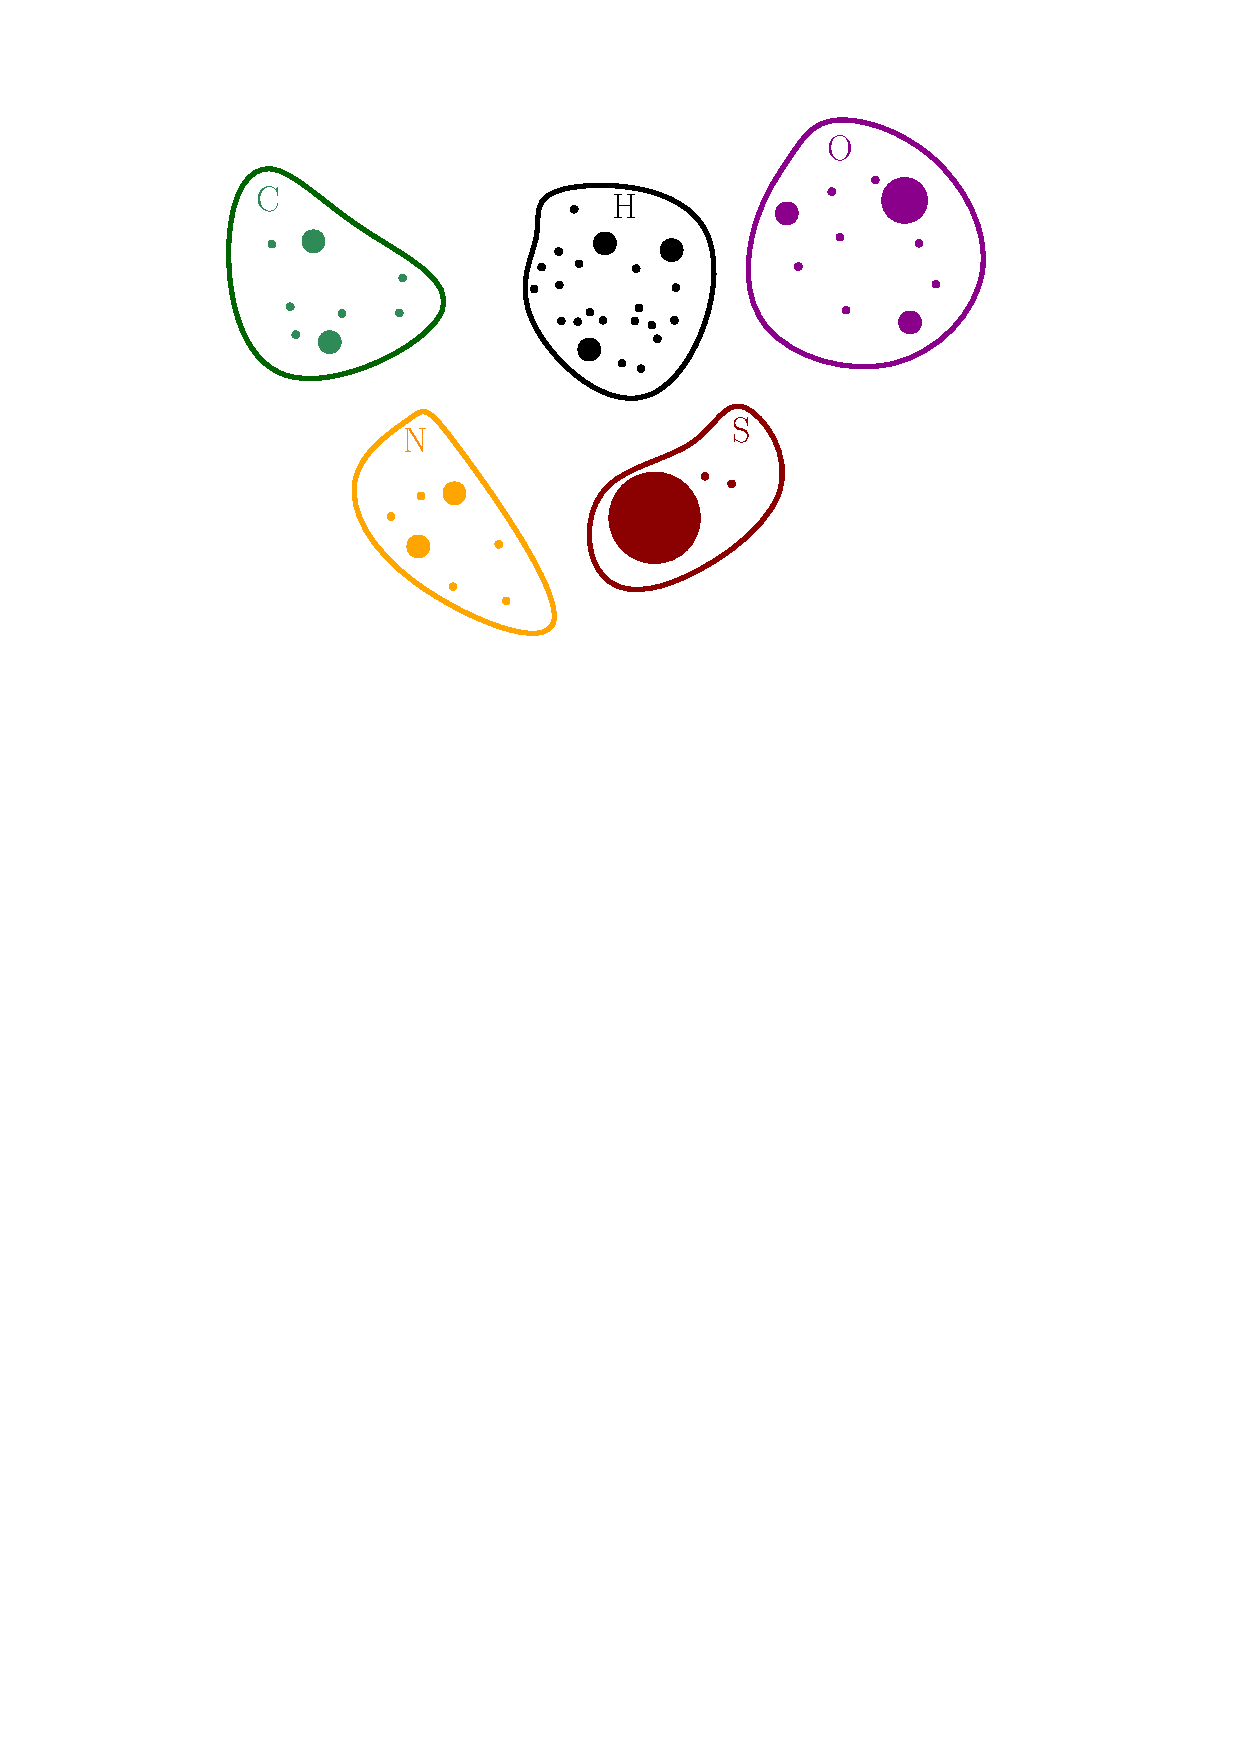
\includegraphics[height=.4\textheight, keepaspectratio]{./picts/molecule.pdf}
		\end{center}

		$$ \prob( 
			\underbrace{\cem{c_{12}} \cem{^{12}C},\, \cem{c_{13}} \cem{^{13}C}}_{\cem{c_{12}}+ \cem{c_{13}} = \cem{c}},\,
			\underbrace{\cem{h_1} \cem{^{1}H},\,\cem{h_2} \cem{^{2}H}}_{\cem{h_1} + \cem{h_2} = \cem{h}}, 
			\,\dots,\, 
			\cem{s_{36}} \cem{^{36}S} ) 
			= 
			$$

		$$ 	{\cem{c} \choose \cem{c_{12}},\cem{c_{13}} }
			\prob(\cem{^{12}C})^{\cem{c_{12}}} \prob(\cem{^{13}C})^{\cem{c_{13}}} 
			{\cem{h} \choose \cem{h_{1}},\cem{h_{2}} }
			\prob(\cem{^{1}H})^{\cem{h_1}} \prob(\cem{^{2}H})^{\cem{h_2}}
			\dots $$	

	\end{frame}


	%%%%%%%%%%%%%%%%%%%%%%%%%%%%%%%%%%%%%%%%%%%%%%%%%%%%%%%%%%%%%%%%%%
	\begin{frame}\frametitle{Multinomial Model and Molecular Mass}
		
		\begin{itemize}
			\item Atomic mass $m$ of a molecule $R = (\cem{c_{12}}, \cem{c_{13}}, \dots \cem{s_{36}})$ 
			\begin{itemize}
				\item[$\star$] $m_R = \cem{c_{12}} m_\cem{^{12}C} + \dots + \cem{s_{36}} m_\cem{^{36}S}$

				\item[$\star$] $\prob(m_R = m) = 
					\sum \prob(
						\cem{c_{12}} \cem{^{12}C}, 
						\dots, 
						\cem{s_{36}} \cem{^{36}S} )$
				\item[s.t.] $m_R = \cem{c_{12}} m_\cem{^{12}C} + \dots + \cem{s_{36}} m_\cem{^{36}S}$
				\item[:)] Good news: theory operates on chemical formulas
				\begin{itemize}
					\item No need to solve these equations!
					\item given a formula $F$, we derive it's mass probability function, $p_F (m)$.	
				\end{itemize}				 
				\item[:(] Bad news 
				\begin{itemize}
					\item The number of peaks grow's quite big this way
				\end{itemize}
			\end{itemize}
			\item Cool thing
			\begin{itemize}
				\item Masses of neutrons for different elements are not equal!
				\item Modern mass specs can already discern them
			\end{itemize}
			\item[$\bigstar$] Neglecting that phenomenon gives rise to BRAIN algorithm
		\end{itemize}



	\end{frame}

	%%%%%%%%%%%%%%%%%%%%%%%%%%%%%%%%%%%%%%%%%%%%%%%%%%%%%%%%%%%%%%%%%%
	\begin{frame}\frametitle{Visualising Multinomial Model}

		\begin{itemize}
			\item BRAIN software - Piotr Dittwald$^\text{\textregistered}$
			\item Assumption: 
			\begin{itemize}
				\item[$\star$]All neutrons have equal masses and cannot be discerned. 
			\end{itemize}
		\end{itemize}

		\begin{columns}
			\begin{column}[t]{.5\textwidth}
				\begin{center}
					Ethanol 
					\ce{C_2 H_5 OH}
					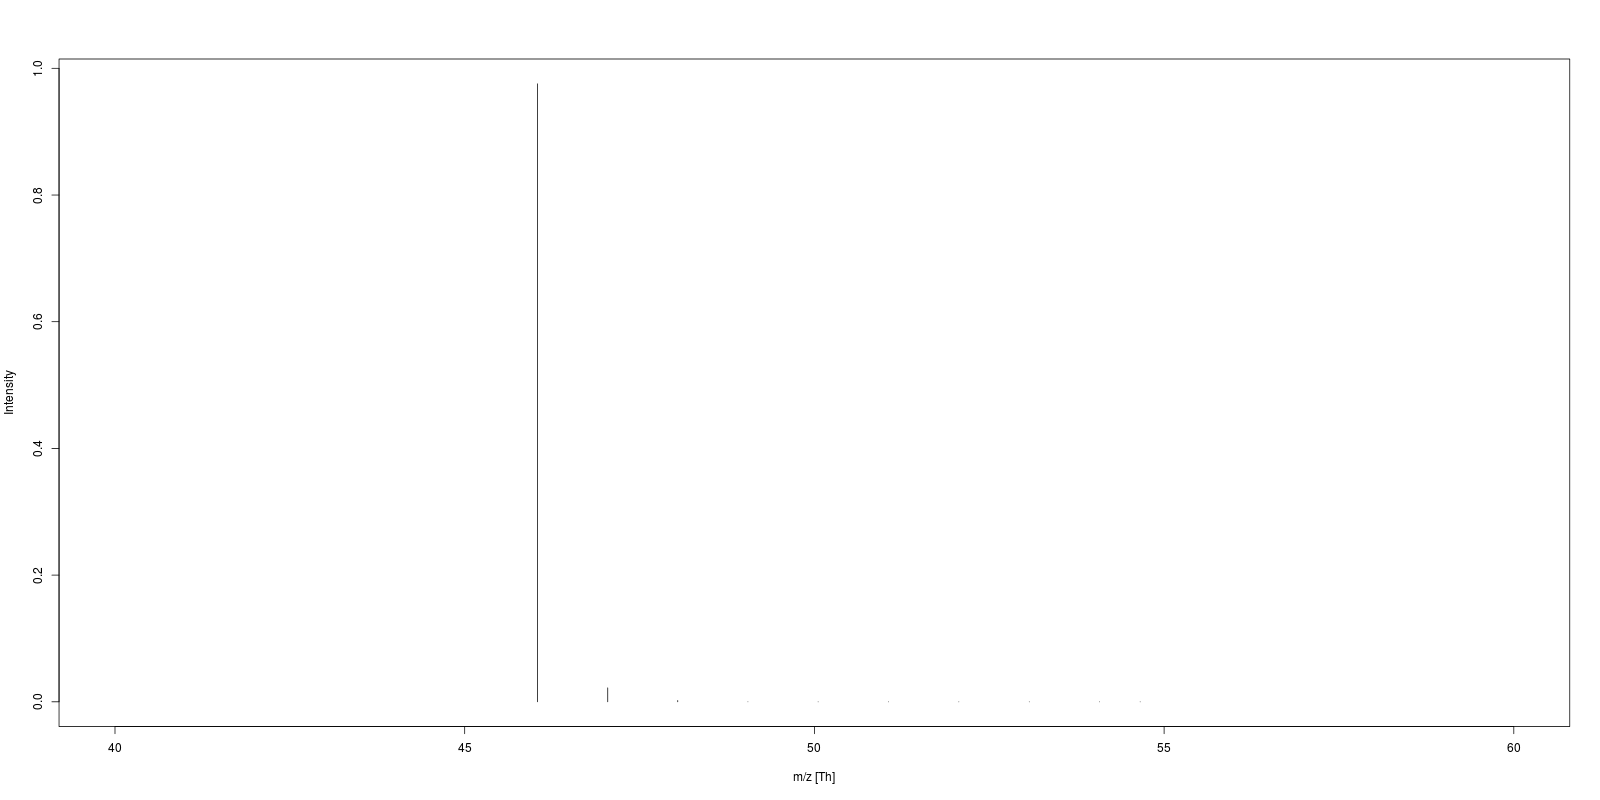
\includegraphics[height=.3\textheight, keepaspectratio]{./picts/ethanol.png}
				\end{center}
			\end{column}
			\begin{column}[t]{.5\textwidth}
				\begin{center}
					Angiotensine II
					\ce{C_{50} H_{71} N_{13} O_{12}}
					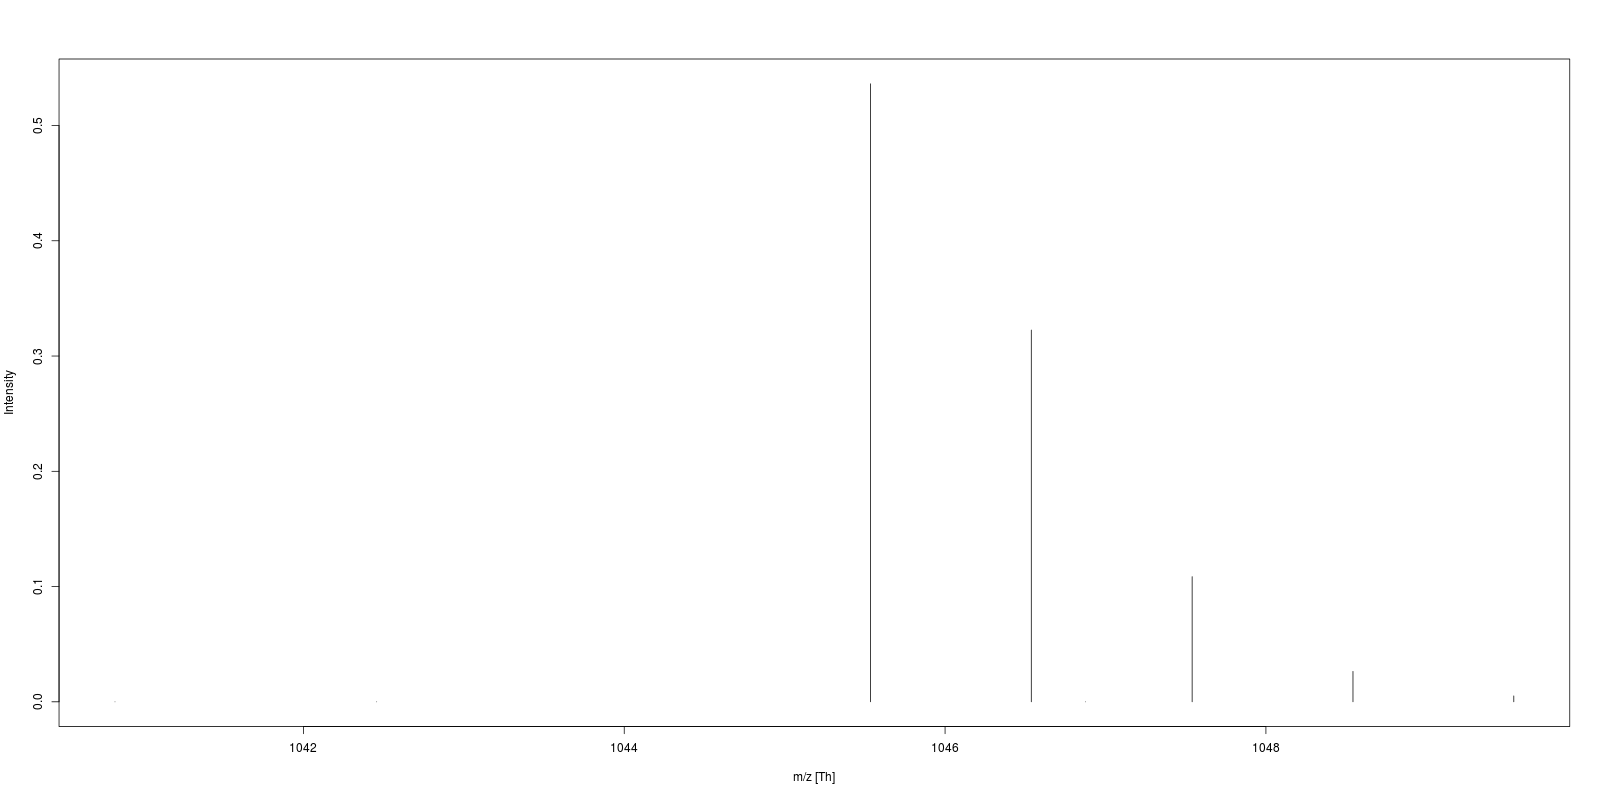
\includegraphics[height=.3\textheight, keepaspectratio]{./picts/angiotensine.png}		
				\end{center}
			\end{column}
		\end{columns}	

		\begin{itemize}
			\item Alas! Real spectra are multimodial!
			\begin{itemize}
				\item fragmentation? (ETD)
				\item charge reductions? (ETD, ETnoD, PTR)
			\end{itemize}
		\end{itemize}
	\end{frame}	

	\framedGraphic{Mass Spec results for substance P}{./picts/inputData.png}

	%%%%%%%%%%%%%%%%%%%%%%%%%%%%%%%%%%%%%%%%%%%%%%%%%%%%%%%%%%%%%%%%%%
	\begin{frame}\frametitle{Polymer as a sequence of Amino Acids}
		\begin{center}
			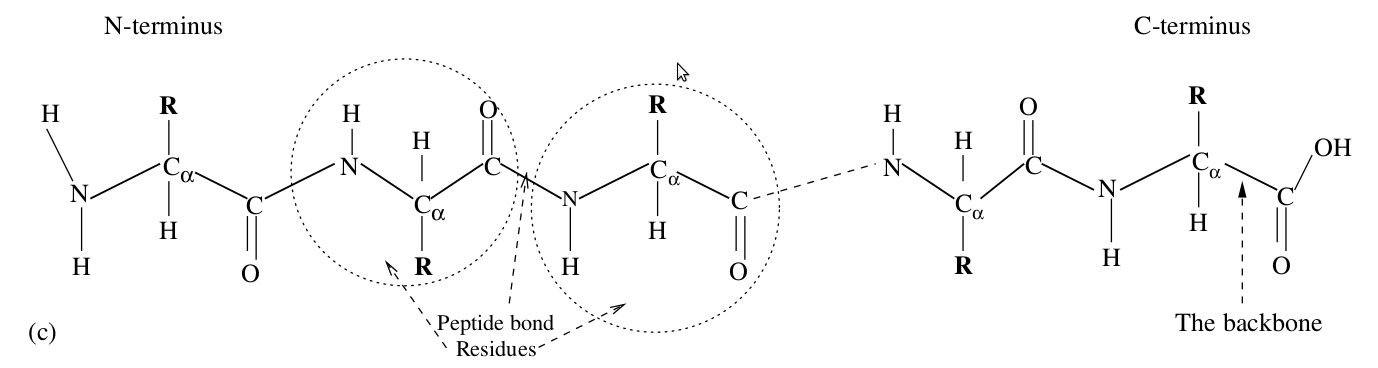
\includegraphics[height=.35\textheight, keepaspectratio]{./picts/aminos.png}
		\end{center}		

		\begin{itemize}
			\item Extra structure in our model must be added
			\begin{itemize}
				\item[] \molecule = $A_1 A_2 \dots A_k$
				\item[] $A_i \in \{ \text{
				Alanine, Cysteine, Aspartic Acid, Glutamic Acid, \dots
				} \}$
			\end{itemize}
		\end{itemize}

	\end{frame}

	\framedGraphic{Molecule Subdivided into Amino Acids}{./picts/moleculeSubdivided.pdf}

	%%%%%%%%%%%%%%%%%%%%%%%%%%%%%%%%%%%%%%%%%%%%%%%%%%%%%%%%%%%%%%%%%%	
	\begin{frame}\frametitle{Electron Transfer Disociation}
		\begin{itemize}
			\item Result: random cleavage of the peptide in two subsequences
			$$ A_1 A_2 \dots A_k \rightarrow 
				\underbrace{A_1 \dots A_L}_\text{$C$ fragment}  \oplus \underbrace{A_{L+1} \dots A_k}_\text{$Z$ fragment}$$
			\item $L$ = index of the cleaved peptide bond (N-terminus to C-terminus) 					
		\end{itemize}

		\begin{columns}
			\begin{column}[t]{.5\textwidth}
				\begin{itemize}
					\item Assumption
				\begin{itemize}
					\item Cleavage independent of isotope composition
					$$ \prob( A_1 \dots A_L = a_1 \dots a_L | L=l ) = 
					$$
					$$ \prob( A_1 \dots A_l = a_1 \dots a_l)$$
				\end{itemize}
					\item Minor complication
					\begin{itemize}
						\item Cleavage solely on $A_1$ 
					\end{itemize}
				\end{itemize}
			\end{column}
			\begin{column}[t]{.5\textwidth}
				\begin{center}
					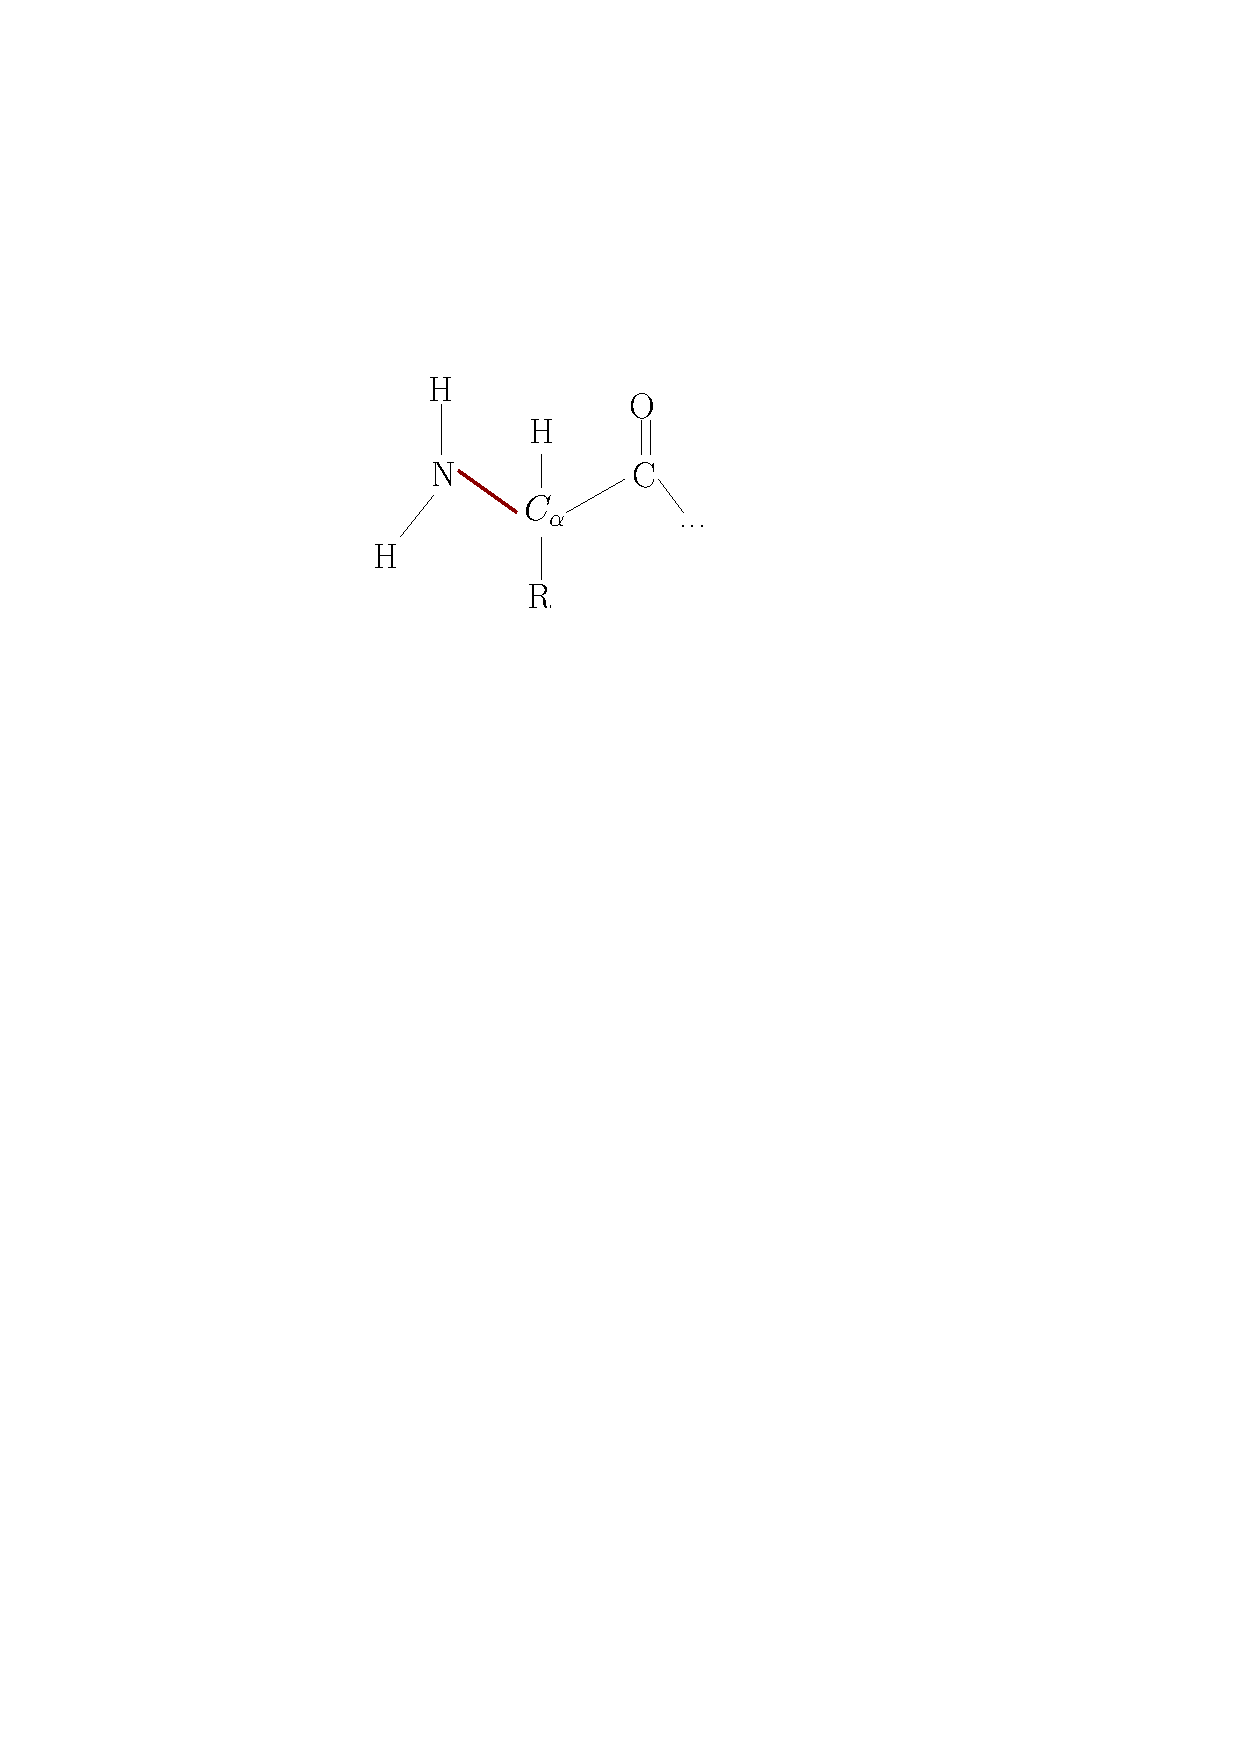
\includegraphics[height=.30\textheight, keepaspectratio]{./picts/aminoAcid.pdf}
				\end{center}
			\end{column}
		\end{columns}
	\end{frame}

	%%%%%%%%%%%%%%%%%%%%%%%%%%%%%%%%%%%%%%%%%%%%%%%%%%%%%%%%%%%%%%%%%%
	\begin{frame}\frametitle{Reactions considered by Frederik, our fellow chemist}
		\begin{itemize}
			\item[] Hypothesis:
			\begin{itemize}
				\item[$\star$] Empirical spectrum = Result of Several Reactions
			\end{itemize}
			\item ETD
			\begin{center}
				\ce{[M $+$ n H]^{n+} + A^{.$-$} -> [C $+$ x H]^{x+} + [Z $+$ (n$-$x)H]^{(n$-$x$-1$).} + A}
			\end{center}
			\item PTR
			\begin{center}
				\ce{[M $+$ n H]^{n+} + A^{.$-$} -> [M $+$ (n$-1$ ) H]^{(n$-1$)+} + AH}
			\end{center}			
			\item ETnoD
			\begin{center}
				\ce{[M $+$ n H]^{n+} + A^{.$-$} -> [M $+$ n H]^{(n$-1$)+.} + A}
			\end{center}			
			\item Not good description of rules
			\begin{itemize}
			 	\item[e.g.] Concatenating reactions: $ETD \rightarrow PTR \rightarrow PTR \rightarrow ETnoD$  
			\end{itemize} 			
		\end{itemize}
	\end{frame}

	%%%%%%%%%%%%%%%%%%%%%%%%%%%%%%%%%%%%%%%%%%%%%%%%%%%%%%%%%%%%%%%%%%
	\begin{frame}\frametitle{Correct Rules}
		
		\begin{itemize}
			\item Additional Description of \molecule - $(p,q)$
			\begin{itemize}
				\item $p$ - protonisation 
				\begin{itemize}
					\item n$^\text{o}$ of extra protons
					\item charge state of a given molecule
					\item adds weight to molecule
				\end{itemize}
				\item $q$ - neutralised protonisation
				\begin{itemize}
					\item n$^\text{o}$ of extra protons paired with electrons
					\item only adds weight
				\end{itemize}				
			\end{itemize}
			\item Problem Input $(A_1 A_2 \dots A_k, p , q)$ 
		\end{itemize}
	\end{frame}

	%%%%%%%%%%%%%%%%%%%%%%%%%%%%%%%%%%%%%%%%%%%%%%%%%%%%%%%%%%%%%%%%%%
	\begin{frame}\frametitle{Reactions revised: post-doc in accountancy}
		
		\begin{itemize}
			\item Problem Input $(A_1 A_2 \dots A_k,\, p ,\, q)$ 
			\item Some Partial Reactions
				\begin{itemize}
				\item[$\clubsuit$] ETD
				\begin{itemize}
					\item[$\rightarrow$] $ (A_1 \dots A_L,\, p_1,\, q_1) $
					\item[$\rightarrow$] $ (A_{L+1} \dots A_k,\, p_2,\, q_2) $
					\item[s.t.]$p_1 + p_2 = p -1$ and $q_1 + q_2 = q$ and $q_2 \geq 0$
				\end{itemize}
				\item[$\diamondsuit$] PTR 
				\begin{itemize}
					\item[$\rightarrow$] $ (A_1 \dots A_k,\, p-1,\, q)$ 
				\end{itemize}
				\item[$\heartsuit$] ETnoD 
				\begin{itemize}
					\item[$\rightarrow$] $ (A_1 \dots A_k,\, p-1,\, q+1)$ 
				\end{itemize}
				\item[$\spadesuit$] \emph{HTR}
				\begin{itemize}
					\item[$\rightarrow$] $ (A_1 \dots A_L,\, p_1,\, q_1)$ 
					\item[$\rightarrow$] $ (A_{L+1} \dots A_k,\, p_2,\, q_2)$ 
					\item[s.t.] $p_1 + p_2 = p$ and $q_1 + q_2 = q + 1$ and $q_2 \geq 1$
				\end{itemize}	
			\end{itemize}
		\end{itemize}
	\end{frame}

	%%%%%%%%%%%%%%%%%%%%%%%%%%%%%%%%%%%%%%%%%%%%%%%%%%%%%%%%%%%%%%%%%%
	\begin{frame}\frametitle{Algorithm?}

		\begin{itemize}
			\item Inputs:
			\begin{itemize}
				\item $S = \Big[M = A_1 \dots A_k,\, p = \text{Maximal Charge}, q = 0\Big]$
				\item Partial Reactions $ = $ 
					$$ = \{ 
					\mathfrak{Id},\,
					\clubsuit^C_{L , p_1, q_1},\,
					\clubsuit^Z_{L,p_2, q_2},\, 
					\diamondsuit,\, 
					\heartsuit,\, 
					\spadesuit^C_{L,\tilde{p}_1, \tilde{q}_1},\, 
					\spadesuit^Z_{L,\tilde{p}_2, \tilde{q}_2} \} $$
				\item Reactions $=$ 
					$$= \{ r_1 r_2 \dots r_k : r_i \text{ is a Partial Reactions and is OK} \} $$
				\item[e.g.] $\clubsuit^C_{L, 2,1} \heartsuit$, $\heartsuit \diamondsuit$ might be valid reactions if 
				\begin{itemize}
					\item $S$ has enough charges
					\item $M$ long enough
					\item there were $q$ reactions before ET resulting in proton neutralisation
				\end{itemize}
				\item Empirical Spectrum, $y = \Big\{ (\frac{m_j}{z_j}, I_j) \Big\}_{j = 1}^{J}$
			\end{itemize}
		\end{itemize}
	\end{frame}

	%%%%%%%%%%%%%%%%%%%%%%%%%%%%%%%%%%%%%%%%%%%%%%%%%%%%%%%%%%%%%%%%%%
	\begin{frame}\frametitle{Deriving many probability functions}
		\begin{itemize}
			\item Observations:
			\begin{itemize}
				\item Each reaction is also a triplet $R = [ F, p, q]$ 
				\item $F \sim$ Multinomial Distribution 
				\item $m_F$ - corresponding mass distribution
				$$ \prob\Big(\frac{m_R}{z_R}\Big)  = \prob\Big(\frac{m_F + p + q}{p}\Big) = p_F (m_F)$$
				\item Some reactions give the same results
				$$\heartsuit \diamondsuit = \diamondsuit \heartsuit$$
				\begin{itemize}
					\item The problem is static: we do not model time explicitly. 
					\item Discernible Reactions $\subset$ Reactions
					\item Reactions $:=$ Equivalence Classes within Reactions 
				\end{itemize}
			\end{itemize}
		\end{itemize}
	\end{frame}

	\framedPlainGraphic{width=\textwidth}{./picts/spectraShifts.png}
	%%%%%%%%%%%%%%%%%%%%%%%%%%%%%%%%%%%%%%%%%%%%%%%%%%%%%%%%%%%%%%%%%%
	\begin{frame}\frametitle{Precising Hypothesis} 
		\begin{itemize}
			\item Empirical Spectrum, $y = \Big\{ (\frac{m_j}{z_j}, I_j) \Big\}_{j = 1}^{J}$
			\item[] Hypothesis
			\begin{itemize}
				\item[$\star$] $I_j = \sum_{R \in \text{Reactions}} \alpha_R \prob(\frac{m_R}{z_R}) + \text{Error}$
				\item[s.t.] $\alpha_R \geq 0,$ 
				\item[] $\sum_R \alpha_R \leq 1$
			\end{itemize}
			\item[]
			\item Problem: need software that
			\begin{itemize}
				\item finds Reactions 
				\item estimates $\alpha_R$ so that error is smallest possible
			\end{itemize}
		\end{itemize}
	\end{frame}

%%%%%%%%%%%%%%%%%%%%%%%%%%%%%%%%%%%%%%%%%%%%%%%%%%%%%%%%%%%%%%%%%%
\section[Fitting]{Fitting Procedures}	

	\framedPlainGraphic{width=\textwidth}{./picts/spectraShiftsAndWeights.png}
%%%%%%%%%%%%%%%%%%%%%%%%%%%%%%%%%%%%%%%%%%%%%%%%%%%%%%%%%%%%%%%%%%

	\begin{frame}\frametitle{massTodon}
		\begin{itemize}
			\item The prototype of the software already exists
			\item Codename - \textsc{massTodon}
			\item Stupid fitting procedure: does not use BRAIN
		\end{itemize}
	\end{frame}

	%%%%%%%%%%%%%%%%%%%%%%%%%%%%%%%%%%%%%%%%%%%%%%%%%%%%%%%%%%%%%%%%%%
	\begin{frame}\frametitle{Kernelisation}

		\begin{itemize}
			\item $y = \Big\{ (\frac{m_j}{z_j}, I_j) \Big\}_{j = 1}^{J}$
			\item Consider a function
				$$ y(z) = \sum_{j=1}^J I_j \times y_j (z)$$
			\begin{itemize}
			 	\item[s.t.]$y_j (z) = \frac{1}{\sqrt{\pi \sigma^2}} e^{-\frac{(z-\mu)^2}{\sigma^2}}$ 
			 	\item[]$\mu = \frac{m_j}{z_j}$
			\end{itemize} 
		\end{itemize}
	\end{frame}

	\framedPlainGraphic{width=\textwidth}{./picts/kernelisation.png}

	%%%%%%%%%%%%%%%%%%%%%%%%%%%%%%%%%%%%%%%%%%%%%%%%%%%%%%%%%%%%%%%%%%
	\begin{frame}\frametitle{Gaussian Approximation to Multinomial Model}

		\begin{itemize}
			\item[] Human Dynein: \ce{C_{23832} H_{37816} N_{6528} O_{7031} S_{170}}			
		\end{itemize}

		\begin{center}
			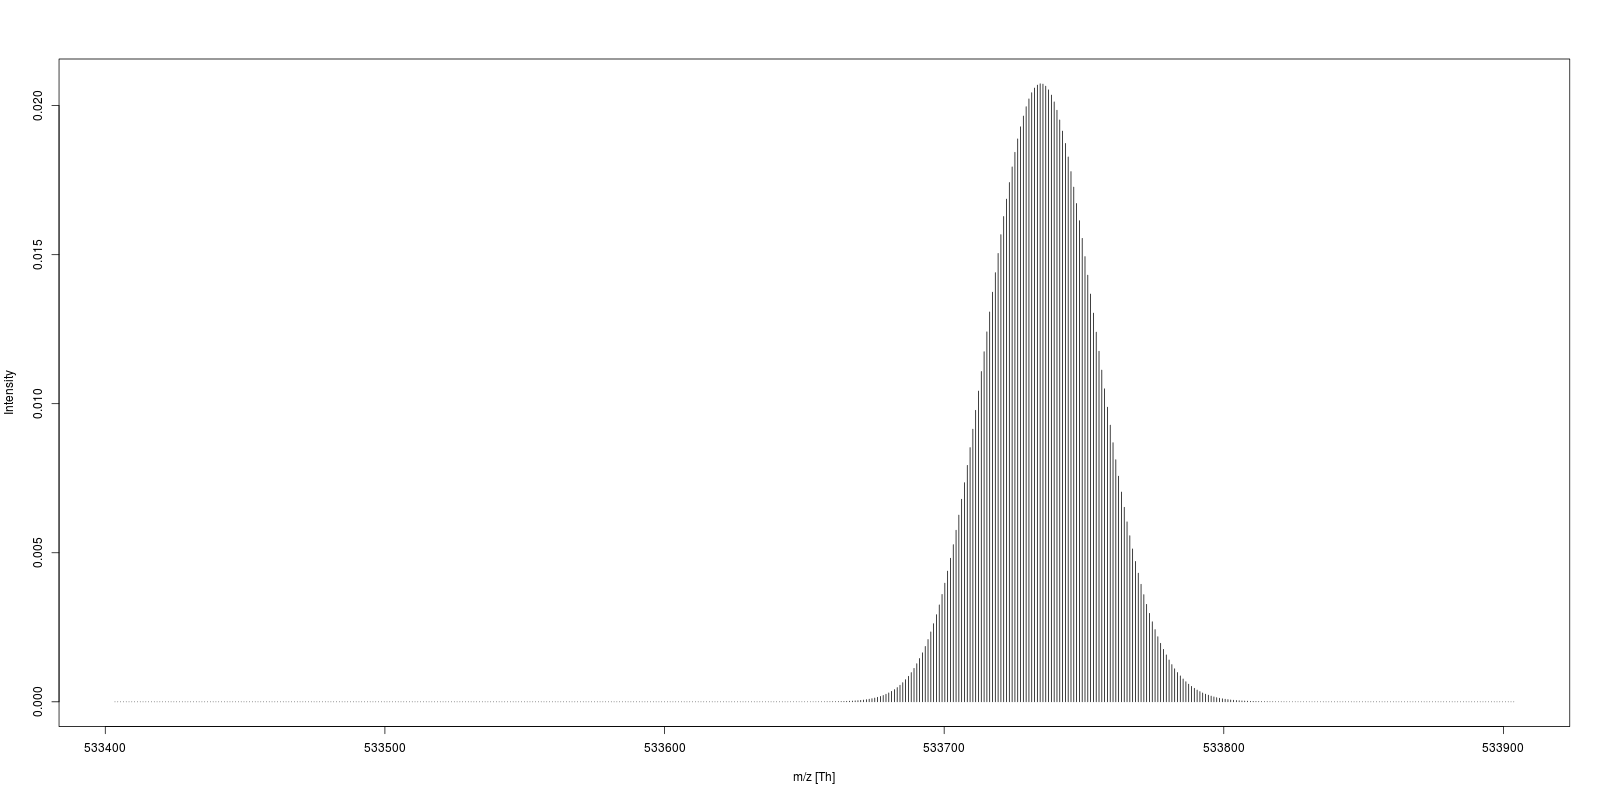
\includegraphics[width=.8\textwidth, keepaspectratio]{./picts/humanDynein.png}
		\end{center}
	\end{frame}

	%%%%%%%%%%%%%%%%%%%%%%%%%%%%%%%%%%%%%%%%%%%%%%%%%%%%%xetex%%%%%%%%%%%%%
	\begin{frame}\frametitle{Gaussian Approximation to Multinomial Model}

		\begin{itemize}
			\item Theoretical Spectra: $\Big\{ f_R(z) \Big\}_{R \in \text{Reactions}}$
			\item Empirical Spectrum: $y(z)$
			\item Linear model:
			$$ y(z) = \sum_{R} \alpha_R f_R (z) + \epsilon(z)$$
			\item Usual least squares humbug
			$$ ||\epsilon||^2 = \Big|\Big| y - \sum_{R} \alpha_R f_k \Big|\Big|^2 \rightarrow \min$$
			\begin{itemize}
				\item[s.t.] $\alpha_R \geq 0$
				\item[s.t.] $\sum_R \alpha_R \leq 1$
				\item[where] $ ||y||^2 = \sprod{y}{y} =  \int_\real y(x)^2 \mathrm{d}\,x.$ 
			\end{itemize}
		\end{itemize}
	\end{frame}

	%%%%%%%%%%%%%%%%%%%%%%%%%%%%%%%%%%%%%%%%%%%%%%%%%%%%%xetex%%%%%%%%%%%%%
	\begin{frame}\frametitle{Gaussian Approximation to Multinomial Model}

		$$ \Big|\Big| y - \sum_{R} \alpha_R f_k \Big|\Big|^2 = || y ||^2 - 2 \alpha^\tran \mathfrak{m} + \alpha^\tran \mathfrak{H} \alpha$$ 

		\begin{itemize}
			\item[where] $\mathfrak{m}^\tran = [ \dots, \sprod{y}{f_R}, \dots ]$
			\item[and] $\mathfrak{H} = [\sprod{f_R}{f_P}]_{R,P \in \text{Reactions}}$
			\item[] 			
			\item Easy to evaluate scalar product 
			$$ m(z) = \frac{1}{\sqrt{\pi \sigma^2}} e^{-\frac{(z-\mu)^2}{\sigma^2}}\text{ and } 
n(z) = \frac{1}{\sqrt{\pi \eta^2}} e^{\frac{(z-\eta)^2}{\nu^2}}
$$
			$$\sprod{m}{n} = \int_\real m(z)n(z) \mathrm{d}\,z  = \frac{1}{\sqrt{\pi (\sigma^2 + \nu^2)}}e^{-\frac{(\mu-\eta)^2}{\sigma^2+\nu^2}}$$  
			\item This problem is numerically very nice
			\begin{itemize}
				\item The Gramm Matrix is diagonally dominant, well conditioned. 
			\end{itemize}
		\end{itemize}

	\end{frame}

	\framedGraphic{Theoretically Explained Spectrum}{./picts/spectrum.png}
	%%%%%%%%%%%%%%%%%%%%%%%%%%%%%%%%%%%%%%%%%%%%%%%%%%%%%xetex%%%%%%%%%%%%%
\section[Plans]{What remains to be done?}

	\begin{frame}\frametitle{Whole lotta of things to do}
		\begin{itemize}
			\item Algorithmically 
			\begin{itemize}
				\item Optimise generation of Reactions: 
				\begin{itemize}
					\item $\heartsuit \diamondsuit = \diamondsuit \heartsuit$
				\end{itemize}
				\item Calibrate fitting procedures: 
				\begin{itemize}
					\item stick spectra more jazzy among chemists
					\item no-one uses gaussian approximations
				\end{itemize}
				\item Derive quick procedures for stick spectra generation: modify BRAIN.
			\end{itemize}
			\item Experimentally
			\begin{itemize}
				\item More substances to analyze
				\item Mixtures of substances 
			\end{itemize}
			\item Pragmatically
			\begin{itemize}
				\item What if the substance is not known?
			\end{itemize}
		\end{itemize}
	\end{frame}

	\begin{frame}\frametitle{massTodon potential}
		\begin{itemize}
			\item Understanding ETD statics
			\item Next step : understand dynamics
			\item Quantitative approach : potential characterisation of peptides through the use of MASS SPEC.
			\begin{itemize}
				\item But not certain yet how to do it yet
			\end{itemize}

		\end{itemize}
	\end{frame}

%%%%%%%%%%%%%%%%%%%%%%%%%%%%%%%%%%%%%%%%%%%%%%%%%%%%%%%%%%%%%%%%%%%%%%%%%%%%%%%%%%%%%%%%%%%%%%%%%%%%%%%%

	
	    
	\begin{thebibliography}{10}

		\beamertemplatebookbibitems
		
		\bibitem{computationalMethodsForMassSpec}
			Ingvar Eidhammer, Kristian Flikka, Lennart Martens, Svein-Ole Mikalsen,
			\emph{Computational Methods for Mass Spectrometry Proteomics}.
			Wiley-Interscience, 
			2007.
			
		\bibitem{computationalMethodsForMassSpec}
			Igor Kaltashov, Stephen J. Eyles
			\emph{Mass Spectrometry in Biophysics: Conformation and Dynamics of Biomolecules}.
			Wiley-Interscience, 
			2005.	
				
	\end{thebibliography}	

	% \begin{frame}[t]\frametitle{Bibliography}
	% 	\bibliographystyle{eccaNoNotes}
	% 	\bibliography{myBooks}
	% \end{frame}


	%%%%%%%%%%%%%%%%%%%%%%%%%%%%%%%%%%%%%%%%%%%%%%%%%%%%%%%%%%%%%%

\end{document}
  
  
%%%%%%%%%%%%%%%%%%%%%%%%%%%%%%%%%%%%%%%%%%%%%%%%%%%%%%%%%%%%%%%%%%%%%%%%%%%

